\ZbSec{Admin} \label{sec:admin}
Im Folgenden wird der Admin Sicht beschrieben. Diese ist eine Ergänzung zur Client Sicht, welche von Herrn Grubauer erstellt wird. Die Datenübertragung des Admin Logins erfolgt dabei über die API, welche von Herrn Mayrhofer erstellt wird. Mehr Informationen über die Admin-Sicht können hier erhalten werden. \ref{subsec:thero:admin}

\newpage

\subsection{Wie meldet man sich als Admin an?}
Die Admin Anmeldung erfolgt über den Login – Sicht von Herrn Grubauer. Dort kann der jeweilige Admin ganz normal seine Mail und Passwort angeben, dann wird dieser über Microsoft authentifiziert. Wenn der Benutzer erfolgreich angemeldet wurde, befindet sich dieser in der Client Sicht. Von dort kann er ganz normale Dinge wie ein normaler Benutzer tun. Wenn sich aber um einen Admin handelt, taucht in der AppBar ein neuer Button auf, mit dem es möglich ist in die Admin Sicht zu gelangen. Dieser Button ist nur für Admins ersichtlich. Wenn der Button gedrückt wurde, befindet sich der jeweilige User dann in der Admin Sicht und kann die bereits vorher beschriebenen Funktionen nutzen. Wenn der Admin dann zurück in die Client Sicht möchte, gibt es ebenfalls in der App Bar einen Button zurück zur Client Sicht. Abmelden ist in den Einstellungen möglich, von dort gelangt der Benutzer wieder zur Login Sicht.

\vspace{0.5cm}
\begin{table}[htbp]
  \centering
  \begin{tabular}{cc}
    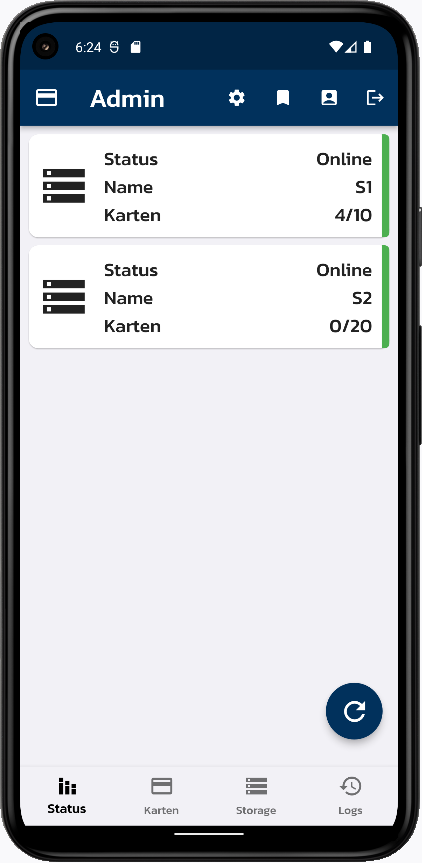
\includegraphics[width=0.35\textwidth]{FLUTTER/images/ZB/status_page.png} & 
    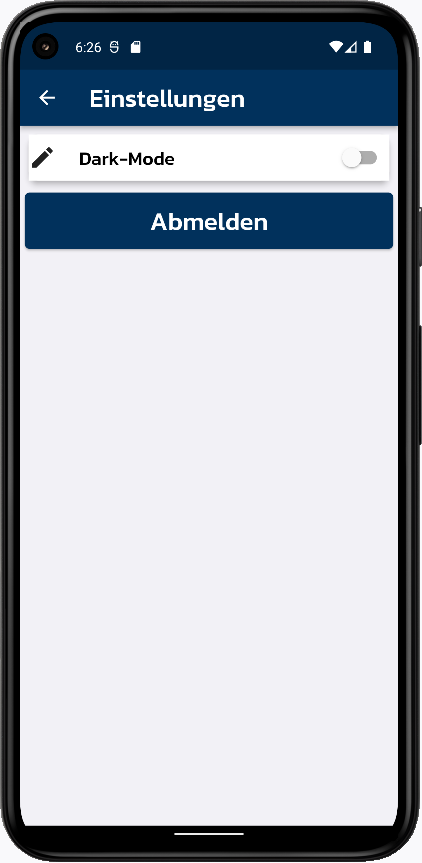
\includegraphics[width=0.35\textwidth]{FLUTTER/images/ZB/settings_page.png} \\
  \end{tabular}
  \label{tab:example}
  \captionsetup{type=figure}
  \caption{Admin Sicht wechseln}
\end{table}

\newpage

\subsection{Navigation in der App}
Die Navigation in der Admin Sicht gestaltet sich als sehr einfach. Wenn der jeweilige Admin Benutzer in der Admin Sicht ist, findet er sich auf der Status-Seite vor. Von dort aus kann er zu allen anderen Seiten gelangen. Am oberen Rand der App befindet sich die App Bar. Über diese kann der Admin zu diversen Funktionen gelangen. Es ist ihm möglich in die Einstellungen zu gehen, die Reservierung-Seite aufzurufen, die User Seite zu besuchen oder sich einfach abzumelden. Alle weiteren von Funktionen sind über die Navigationsleiste am unteren Rand der Seite zugänglich. Von dort kann der Admin die Status-Seite aufrufen, in der er sich bereits befindet, die Cards Seite besuchen, die Storage Seite aufrufen oder zur Log Seite wechseln.

\vspace{1cm}
\begin{table}[htbp]
  \centering
  \begin{tabular}{cc}
    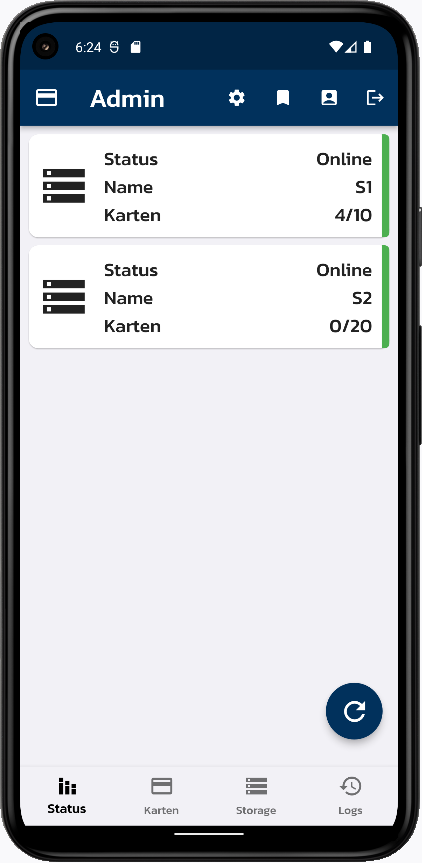
\includegraphics[width=0.37\textwidth]{FLUTTER/images/ZB/status_page.png} \\
  \end{tabular}
  \label{tab:example}
  \captionsetup{type=figure}
  \caption{Navigation in der App}
\end{table}

\newpage

\subsection{Daten neu laden}
Wenn der Administrator Änderung an den Daten vorgenommen hat, sei es neue Karte anlegen oder Bearbeiten, selbiges Spiel auch für alles andere, muss über den Reload Button in rechten unteren Ecke die Daten neu geladen werden. Dabei wird im Hintergrund ein API Aufruf durchgeführt, damit die Daten aktuell sind.

\vspace{1cm}
\begin{table}[htbp]
  \centering
  \begin{tabular}{cc}
    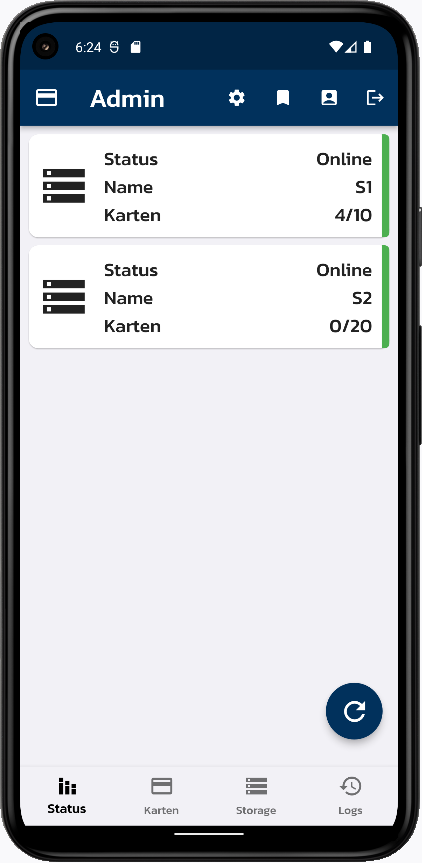
\includegraphics[width=0.4\textwidth]{FLUTTER/images/ZB/status_page.png}  \\
  \end{tabular}
  \label{tab:example}
  \captionsetup{type=figure}
  \caption{Daten neu laden}
\end{table}

\newpage

\subsection{Funktionen der Admin – Sicht}
Die Admin Sicht bietet eine hohe Flexibilität, Storages und deren Karten zu verwalten. Des Weiteren lassen sich Benutzer und Reservierungen verwalten. sowie Logs und Statistiken anzeigen. Im Folgenden werden all diese Funktionen genauer erläutert:

\subsection{Status}
Wenn sich der jeweilige User erfolgreich über die Login Sicht angemeldet hat und über er die Einstellungsseite in die Admin Sicht gelangt ist, wird er von der Status-Seite begrüßt. Diese soll einen kurzen Überblick über den aktuellen Stand der Karten Tresore bieten. Dem Admin wird angezeigt, ob der jeweilige Storage Online ist, wie viele Karten aktuell vorhanden sind. Wenn der Admin auf den jeweiligen Storage drückt, werden ihm einige Optionen angezeigt, welche er durchführen kann.
\vspace{3cm}
\\
\vspace{3cm}
\textbf{Ping Storage} \ref{subsubsec:ping}
\\
\vspace{3cm}
\textbf{Focus Storage} \ref{subsubsec:focus}
\\
\vspace{3cm}
\textbf{Karten Statistik} \ref{subsubsec:stats}

\newpage

\subsubsection{Focus} \label{subsubsec:focus}
Über die Focus Option kann der Administrator den Storage ins System  aufnehmen. Das heißt, wenn der Admin auf der Storage Seite den neuen Tresor angelegt hat, wird dieser Rot markiert angezeigt. Das soll dem Admin mitteilen, dass er den Storage noch ``Focusen`` muss. Dazu geht dieser auf die Status-Seite, drückt auf den Storage. Danach wählt er die Option ``Focus`` und der Storage wird in das System aufgenommen. Jetzt ist es auch möglich, Karten in diesem Tresor anzulegen.

\vspace{1cm}
\begin{table}[htbp]
  \centering
  \begin{tabular}{cc}
    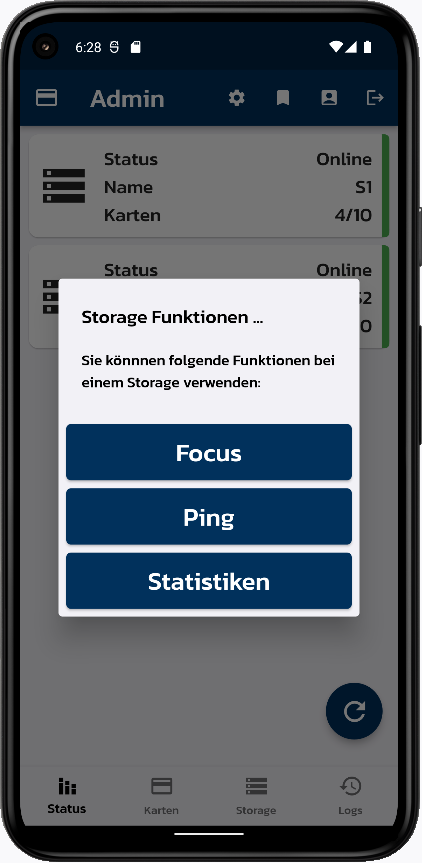
\includegraphics[width=0.4\textwidth]{FLUTTER/images/ZB/status_page_selector.png} &
    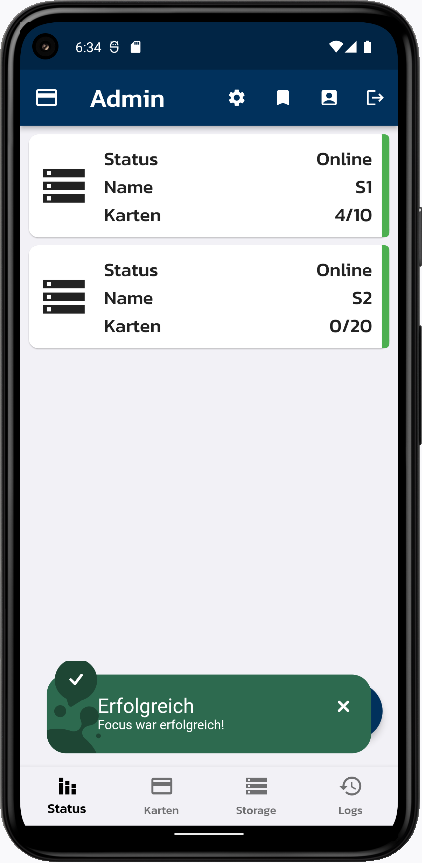
\includegraphics[width=0.4\textwidth]{FLUTTER/images/ZB/status_focus_storage.png} \\
  \end{tabular}
  \label{tab:example}
  \captionsetup{type=figure}
  \caption{Focus Storage}
\end{table}

\newpage

\subsubsection{Ping} \label{subsubsec:ping}
Mittels der Ping Option wird dem Admin die Möglichkeit geboten, zu überprüfen, ob ein Karten Tresor Online oder Offline ist. Dies kann er dadurch durchführen, in dem er auf der Status-Seite auf den Karten Tresor klickt und die Option Ping auswählt. Dabei wird im Hintergrund über die API ein Ping ausgeführt und wenn der Storage erreicht werden kann, wird dies dem User angezeigt. Wenn nicht, dann natürlich nicht. Der User braucht den Ping aber nicht unbedingt manuell durchzuführen, da bereits auf der Status-Seite bei allen Storages angezeigt wird, ob diese ``Ping bar`` waren.

\vspace{1cm}
\begin{table}[htbp]
  \centering
  \begin{tabular}{cc}
    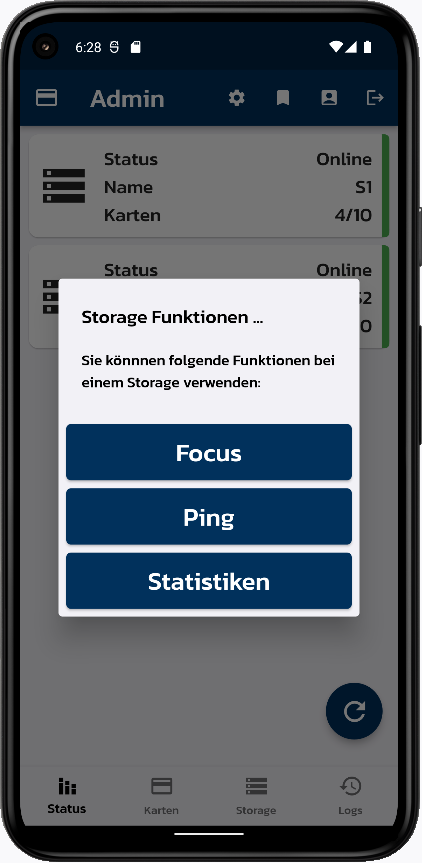
\includegraphics[width=0.4\textwidth]{FLUTTER/images/ZB/status_page_selector.png} &
    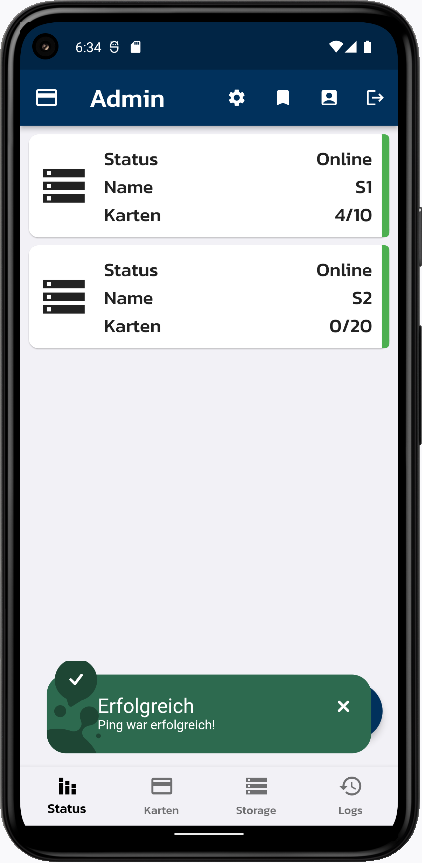
\includegraphics[width=0.4\textwidth]{FLUTTER/images/ZB/status_ping_storage.png} \\
  \end{tabular}
  \label{tab:example}
  \captionsetup{type=figure}
  \caption{Ping Storage}
\end{table}

\newpage

\subsubsection{Statistik} \label{subsubsec:stats}
Die letzte Option, die dem Administrator geboten wird, ist die Statistik Option. Diese ist auch wie die beiden andern auf der Status-Seite zugänglich, wenn man auf den jeweiligen Storage klickt. In der Statistik-Seite werden dem Admin zu allen Karten angezeigt, wie oft diese ausgeborgt wurden. Dies wird natürlich separat pro Karte angezeigt. Dies soll den Admin darüber informiere, ob es vielleicht besser wäre manche Karten auf andere Tresore zu verteilen, da vielleicht bei dem einen sehr hohe ausborge Zahlen zustande kamen und bei einem anderen nur sehr geringe.

\vspace{1cm}
\begin{table}[htbp]
  \centering
  \begin{tabular}{cc}
    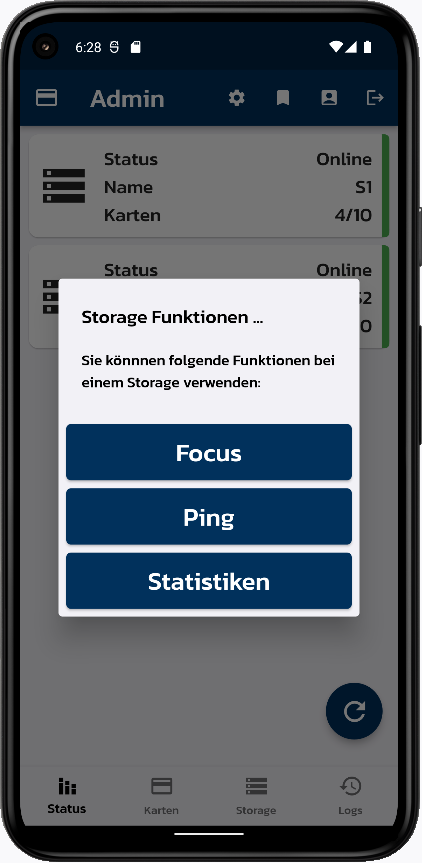
\includegraphics[width=0.4\textwidth]{FLUTTER/images/ZB/status_page_selector.png} &
    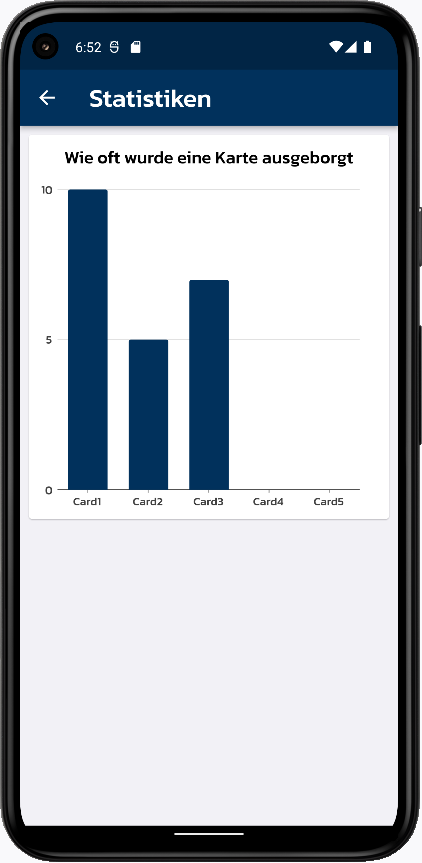
\includegraphics[width=0.4\textwidth]{FLUTTER/images/ZB/stats_page.png} \\
  \end{tabular}
  \label{tab:example}
  \captionsetup{type=figure}
  \caption{Statistik anzeigen}
\end{table}

\newpage

\subsection{Karten} 
Direkt neben der Status-Seite, ist für den Admin die Karten-Seite zu erreichen. Bei dieser kann der Administrator sämtlich Einstellungen, welche Karten betreffen, durchführen. Wenn der Admin auf Seite gelangt, sind im oberen Teil einige Funktionen zugänglich. Der Admin kann neue Karten anlegen. Er kann nach Karten suchen und nach Storages filtern, um schneller zu den gewünschten Karten zu gelangen. Wenn der Admin Einstellungen an Karten vornehmen will, kann er auf eine der aufgelisteten Karten klicken und bekommt zwei Optionen, welche er ausführen kann. Die erste wäre, die Karte zu bearbeiten und die zweite, die jeweilige Karte zu löschen. Des Weiteren, wird bei der Karte angezeigt, in welchem Storage diese sich befinden, wie oft diese verwendet wurden und ob sie gerade verfügbar sind. Der Verfügbarkeit-Status ist auch über die farbige Markierung am Rand ersichtlich.
\vspace{3cm}
\\
\vspace{3cm}
\textbf{Karte hinzufügen} \ref{subsubsec:addCard}
\\
\vspace{3cm}
\textbf{Karte bearbeiten} \ref{subsubsec:alterCard}
\\
\vspace{3cm}
\textbf{Karte löschen} \ref{subsubsec:deleteCard}

\newpage

\subsubsection{Karte – Hinzufügen} \label{subsubsec:addCard}
Wenn der Admin eine neue Karte anlegen möchte, muss dieser lediglich über den Button hinzufügen in die Sicht wechseln. Von dort aus muss dieser lediglich den Namen der Karte und jeweiligen Karten Tresor angeben, in dem die Karte hinterlegt werden soll. \textbf{Bei dem anlegen Vorgang wird überprüft, ob die Karte bereits vorhanden ist und es werden nur Storages angezeigt, welche auch mittels der Option Focus in das System aufgenommen wurden.} Wenn die Daten eingepflegt wurden, muss der Admin lediglich noch auf anlegen klicken und die jeweilige Karte an den Scanner halten, dafür hat er 20 Sekunden Zeit. Wenn keine Karte gescannt wurde, wird der Vorgang abgebrochen.

\vspace{1cm}
\begin{table}[htbp]
  \centering
  \begin{tabular}{cc}
    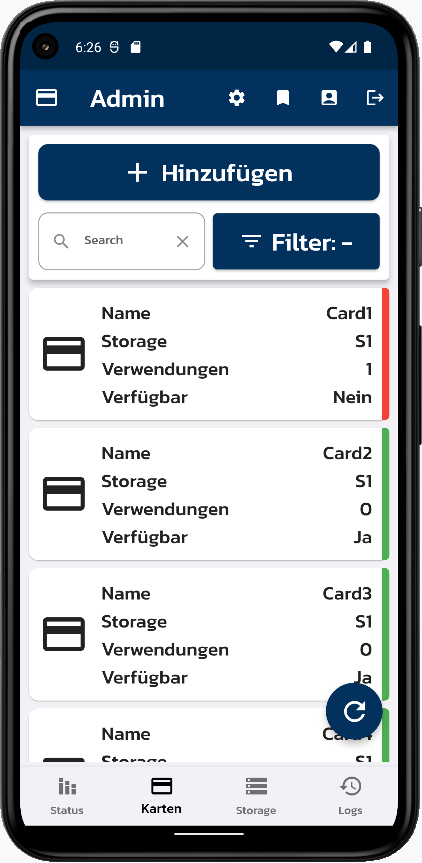
\includegraphics[width=0.37\textwidth]{FLUTTER/images/ZB/card_page.png} &
    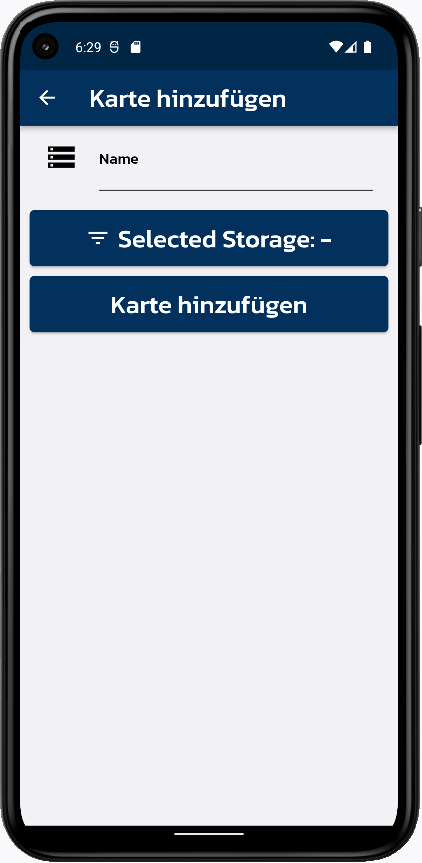
\includegraphics[width=0.37\textwidth]{FLUTTER/images/ZB/card_add_page.png} \\
  \end{tabular}
  \label{tab:example}
  \captionsetup{type=figure}
  \caption{Karte hinzufügen}
\end{table}

\newpage

\subsubsection{Karte – Bearbeiten} \label{subsubsec:alterCard}
Wenn eine Karte im System bearbeitetet, werden soll, kann der Admin dies ebenfalls durchführen. Dazu muss der Admin lediglich auf eine der aufgelisteten Karten klicken und Karte bearbeiten auswählen. Dort kann dieser dann den Namen und den Storage ändern. Es wird ebenfalls geprüft, ob, der Name bereits vorhanden ist.

\vspace{1cm}
\begin{table}[htbp]
  \centering
  \begin{tabular}{cc}
    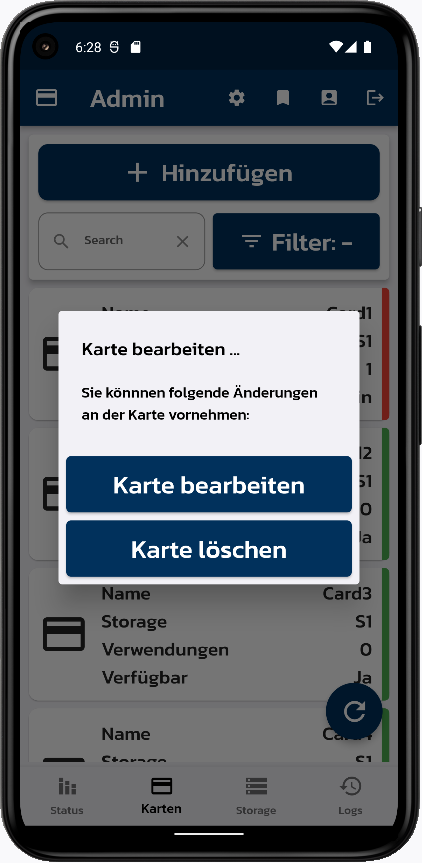
\includegraphics[width=0.4\textwidth]{FLUTTER/images/ZB/card_page_selector.png} &
    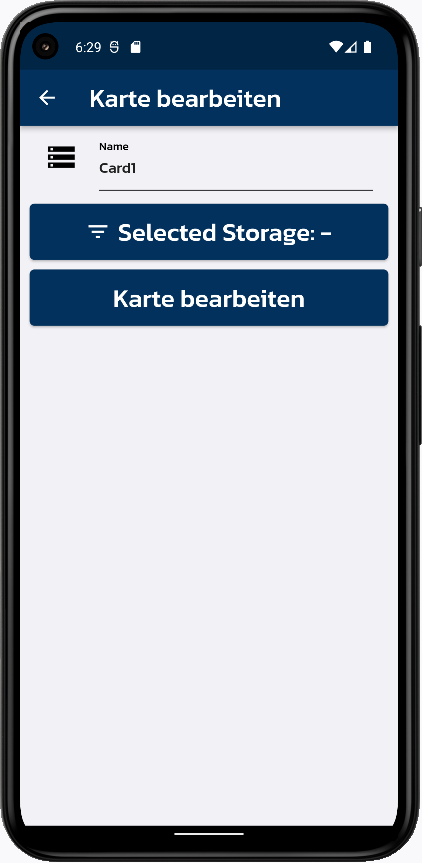
\includegraphics[width=0.4\textwidth]{FLUTTER/images/ZB/card_alter_page.png} \\
  \end{tabular}
  \label{tab:example}
  \captionsetup{type=figure}
  \caption{Karte bearbeiten}
\end{table}

\newpage

\subsubsection{Karte – Löschen} \label{subsubsec:deleteCard}
Eine Karte kann man natürlich auch löschen. Dazu ebenfalls wie bei Karte bearbeiten, auf die jeweilige Karte klicken und die Option Karte löschen wählen. \textbf{Einen Karte kann nur gelöscht werden, wenn keine offenen Reservierungen mehr vorhanden sind.}

\vspace{1cm}
\begin{table}[htbp]
  \centering
  \begin{tabular}{cc}
    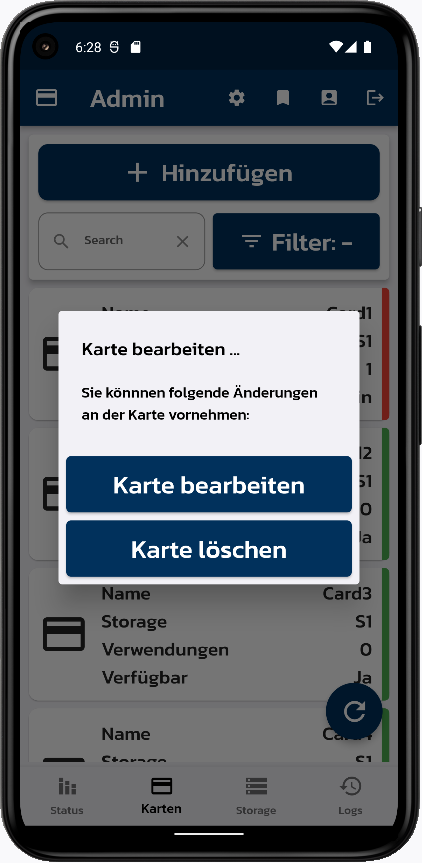
\includegraphics[width=0.4\textwidth]{FLUTTER/images/ZB/card_page_selector.png} &
    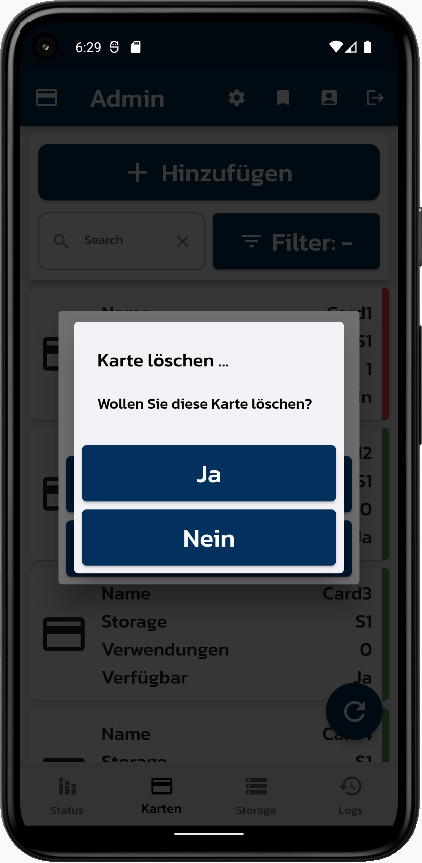
\includegraphics[width=0.4\textwidth]{FLUTTER/images/ZB/card_delete_page.png} \\
  \end{tabular}
  \label{tab:example}
  \captionsetup{type=figure}
  \caption{Karte löschen}
\end{table}

\newpage

\subsection{Storages}
Eine Seite weiter. Von dort aus kann der Admin alles Rund um Storages verwalten. Im oberen Teil der Seite werden dem Admin wieder einige Funktionen geboten. Dazu gehören, neue Storages anzulegen oder nach Storages zu suchen. Wenn ein vorhandener Storage bearbeitetet, werden soll, kann dies über Anklicken des jeweiligen Storages getan werden. Löschen funktioniert ebenfalls identisch. Es wird auch noch angezeigt, ob der jeweilige Storage ``gefocused`` wurde. Dies ist über die farbige Markierung oder die Option Focus ersichtlich. Weiters wird noch die Kapazität und der Ort des jeweiligen Storages angezeigt.
\vspace{3cm}
\\
\vspace{3cm}
\textbf{Storage hinzufügen} \ref{subsubsec:addStorage}
\\
\vspace{3cm}
\textbf{Storage bearbeiten} \ref{subsubsec:alterStorage}
\\
\vspace{3cm}
\textbf{Storage löschen} \ref{subsubsec:deleteStorage}

\newpage

\subsubsection{Storage – Hinzufügen} \label{subsubsec:addStorage}
Wenn der Admin einen neuen Storage anlegen möchte, kann er dies über den oben liegende Option Hinzufügen tun. Dabei muss der Admin den Namen, den Standort und die Anzahl der Karten, welche im Tresor hinterlegt werden können, angeben. \textbf{Es wird natürlich geprüft, ob es bereits einen Tresor mit diesem Namen gibt}. Wenn alles in Ordnung ist, kann über die Option Storage Hinzufügen der Storage angelegt werden. Jetzt muss der Admin lediglich den Storage noch mittels der Funktion \textit{Focus} als aktiv setzten, um Karten anlegen zu können.

\vspace{1cm}
\begin{table}[htbp]
  \centering
  \begin{tabular}{cc}
    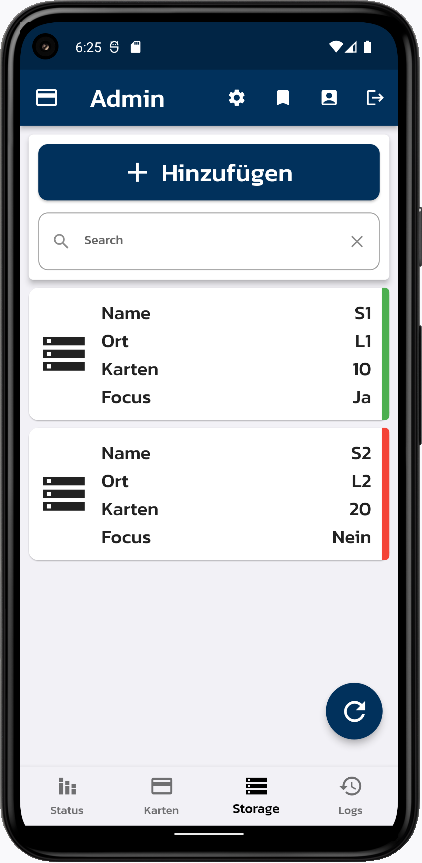
\includegraphics[width=0.4\textwidth]{FLUTTER/images/ZB/storage_page.png} &
    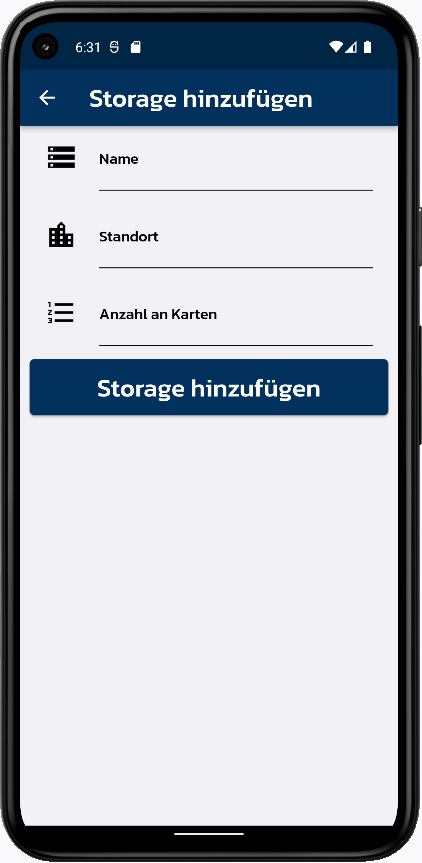
\includegraphics[width=0.4\textwidth]{FLUTTER/images/ZB/storage_add_page.png} \\
  \end{tabular}
  \label{tab:example}
  \captionsetup{type=figure}
  \caption{Schließfach hinzufügen}
\end{table}

\newpage

\subsubsection{Storage – Bearbeiten} \label{subsubsec:alterStorage}
Falls der Fall eintreten sollte, dass ein Tresor bearbeitetet werden muss, kann dies durch Anklicken des jeweiligen Storages erreicht werden. Dort muss dann nur die Option Storage bearbeiten gewählt werden. Von hier aus können dann der Name, der Ort und die Anzahl der Karten verändert werden. Es wird ebenfalls geprüft, ob der Name bereits vorhanden ist.

\vspace{1cm}
\begin{table}[htbp]
  \centering
  \begin{tabular}{cc}
    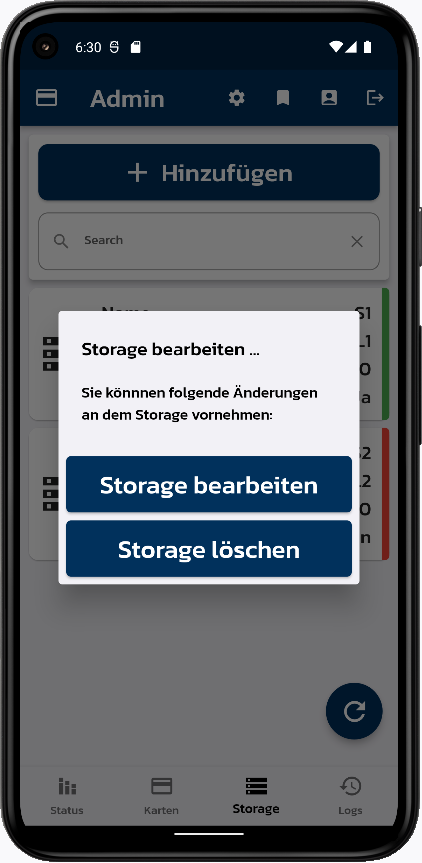
\includegraphics[width=0.4\textwidth]{FLUTTER/images/ZB/storage_page_selector.png} &
    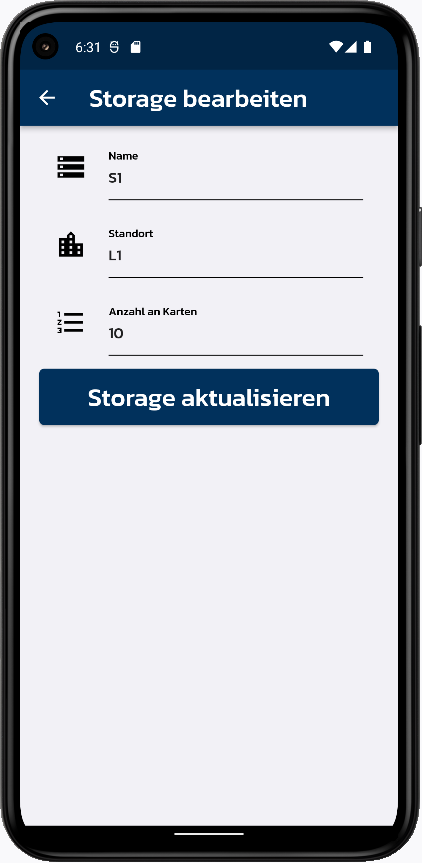
\includegraphics[width=0.4\textwidth]{FLUTTER/images/ZB/storage_alter_page.png} \\
  \end{tabular}
  \label{tab:example}
  \captionsetup{type=figure}
  \caption{Schließfach bearbeiten}
\end{table}

\newpage

\subsubsection{Storage – Löschen} \label{subsubsec:deleteStorage}
Ein Storage kann auch gelöscht werden. Wenn man den Storage löschen möchte, muss der Admin den jeweiligen Storage auswählen und die Option löschen auswählen. \textbf{Wenn der Storage noch mit Karten befüllt ist, kann dieser nicht gelöscht werden. Das selbige gilt, auch wenn diese Karten noch offene Reservierungen haben, müssen diese zuerst gelöscht werden.}

\vspace{1cm}
\begin{table}[htbp]
  \centering
  \begin{tabular}{cc}
    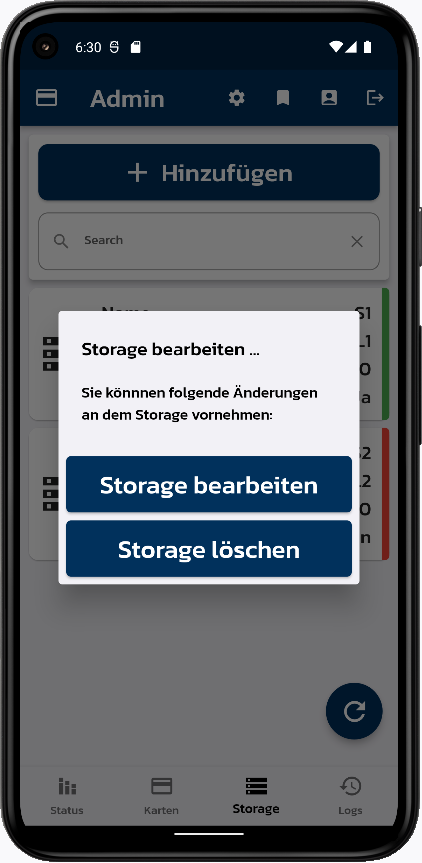
\includegraphics[width=0.4\textwidth]{FLUTTER/images/ZB/storage_page_selector.png} &
    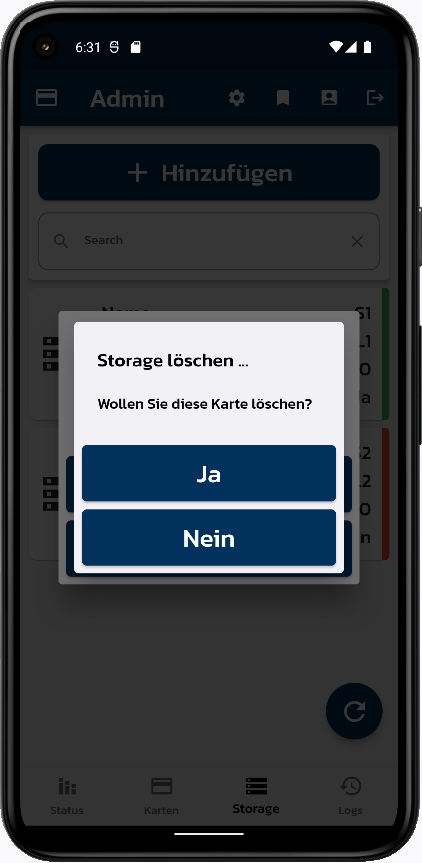
\includegraphics[width=0.4\textwidth]{FLUTTER/images/ZB/storage_delete_page.png} \\
  \end{tabular}
  \label{tab:example}
  \captionsetup{type=figure}
  \caption{Schließfach löschen}
\end{table}

\newpage

\subsection{Logs}
Wenn der User ganz rechts bei den Seiten ankommen ist, wird ihm die Log Seite präsentiert. Diese umfasst alle Aktionen, welche im Hintergrund durchgeführt werden. Diese soll den Admin dabei unterstützen, Fehler finden zu können und diese zu beheben. Die angezeigten Logs bleiben, solange gespeichert, bis der Admin die Admin Sicht verlässt. Das heißt, die App schließt oder zur Client Sicht wechselt.

\vspace{1cm}
\begin{table}[htbp]
  \centering
  \begin{tabular}{c}
    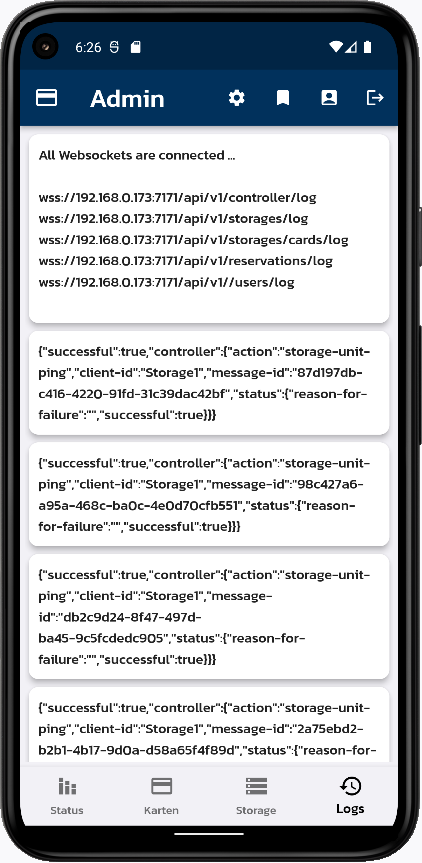
\includegraphics[width=0.4\textwidth]{FLUTTER/images/ZB/logs_page.png} 
  \end{tabular}
  \label{tab:example}
  \captionsetup{type=figure}
  \caption{Logs anzeigen}
\end{table}

\newpage

\subsection{Benutzer}
Über die App Bar am oberen Rand kann der Benutzer noch zu weiteren Funktionen gelangen. Eine davon ist der Benutzer Tab, welcher über das Account Icon zugänglich ist. Von dort aus kann der Admin Benutzer zu einem Admin machen oder diese auch löschen. Dazu stehen ihm auch eine Such leiste breit zum schnellen Finden von Benutzern. In der Liste von Benutzern, wird von jedem die Mail-Adresse und angezeigt, ob der Benutzer schon Admin ist oder nicht.
\vspace{5cm}
\\
\vspace{5cm}
\textbf{Benutzer zu Admin} \ref{subsubsec:userAdmin}
\\
\vspace{5cm}
\textbf{Benutzer löschen} \ref{subsubsec:deleteUser}

\newpage

\subsubsection{Benutzer – Admin}  \label{subsubsec:userAdmin}
Wenn der Admin einen Benutzer zu einem Admin machen möchte, muss er lediglich auf den jeweiligen Benutzer klicken und Berechtigungen ändern drücken. Somit wird der Benutzer zu einem Admin gemacht.

\vspace{1cm}
\begin{table}[htbp]
  \centering
  \begin{tabular}{cc}
    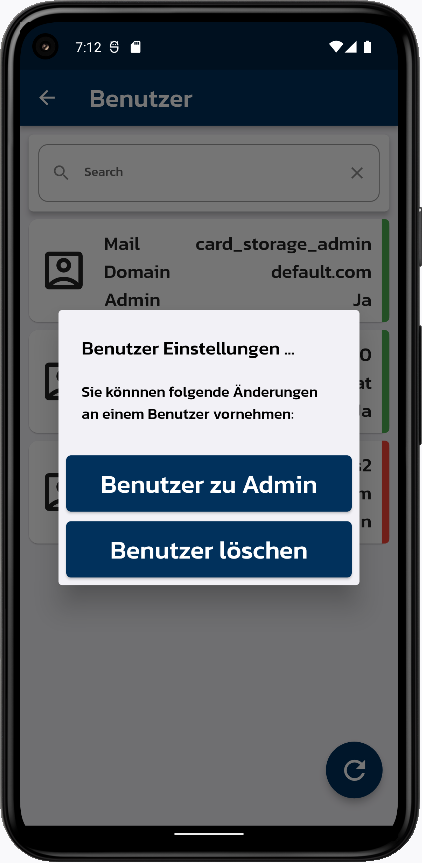
\includegraphics[width=0.4\textwidth]{FLUTTER/images/ZB/user_page_selector.png} &
    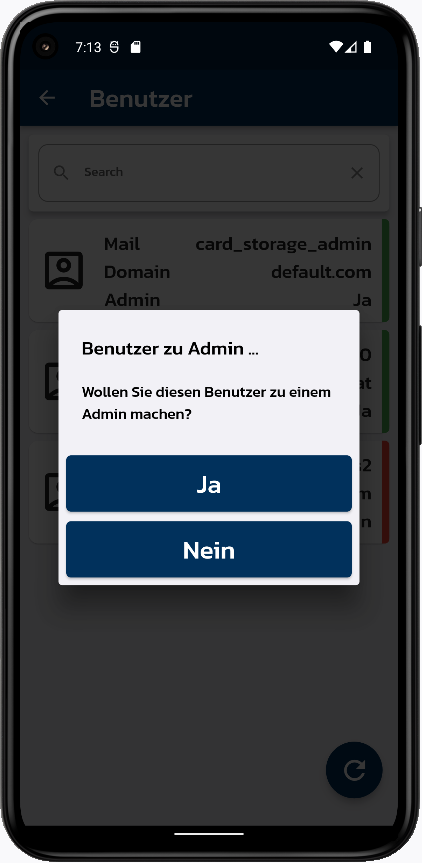
\includegraphics[width=0.4\textwidth]{FLUTTER/images/ZB/user_admin.png} \\
  \end{tabular}
  \label{tab:example}
  \captionsetup{type=figure}
  \caption{Benutzer zu Admin}
\end{table}

\newpage

\subsubsection{Benutzer – Löschen} \label{subsubsec:deleteUser}
Falls ein Benutzer gelöscht werden soll, muss ebenfalls lediglich auf den Benutzer gedrückt werden und die Option löschen gewählt werden. \textbf{Ein Benutzer kann nicht gelöscht werden, wenn er noch offene Reservierungen hat.}

\vspace{1cm}
\begin{table}[htbp]
  \centering
  \begin{tabular}{cc}
    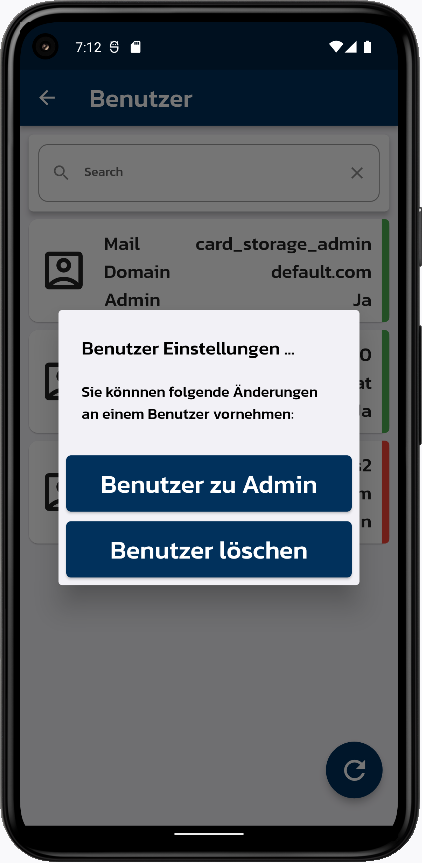
\includegraphics[width=0.4\textwidth]{FLUTTER/images/ZB/user_page_selector.png} &
    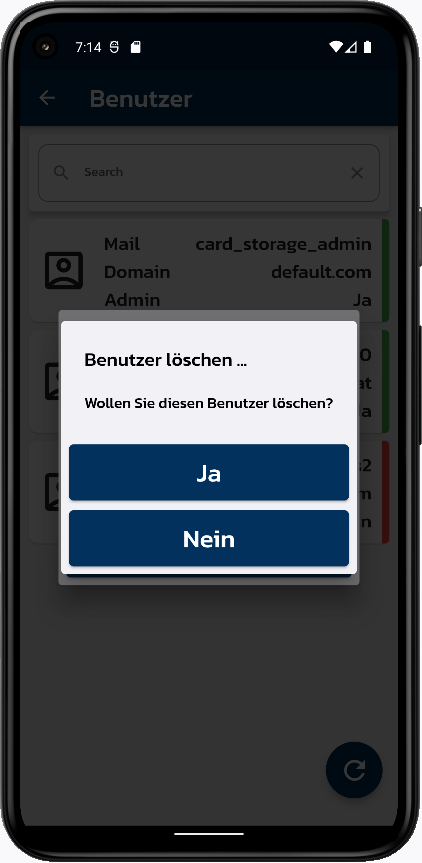
\includegraphics[width=0.4\textwidth]{FLUTTER/images/ZB/user_delete.png} \\
  \end{tabular}
  \label{tab:example}
  \captionsetup{type=figure}
  \caption{Benutzer löschen}
\end{table}

\newpage

\subsection{Reservierungen}
Eine weiter Funktion, welche über die App Bar zugänglich ist, sind die Reservierungen. Diese sind über das Reservierung-Icon zugänglich. Bei der Seite angelegt, kann der Admin nach Reservierungen suchen und löschen, sowie die Zeit einstellen, bis wann vor Ablauf der Reservierung. die Karte nicht mehr abgeholt werden kann. Z. B.: Reservierung läuft bis 17:00, 30 Minuten davor kann die Karte nicht mehr ausgeborgt werden.
\vspace{5cm}
\\
\vspace{5cm}
\textbf{Reservierung löschen} \ref{subsubsec:reservationTime}
\\
\vspace{5cm}
\textbf{Reservierung Zeit} \ref{subsubsec:deleteReservation}

\newpage

\subsubsection{Reservierung - Löschen} \label{subsubsec:deleteReservation}
Falls eine Reservierung gelöscht werden soll, kann dies über Anklicken der jeweiligen Reservierung getan werden. \textbf{Es können natürlich auch noch aktuelle Reservierungen gelöscht werden.}

\vspace{1cm}
\begin{table}[htbp]
  \centering
  \begin{tabular}{cc}
    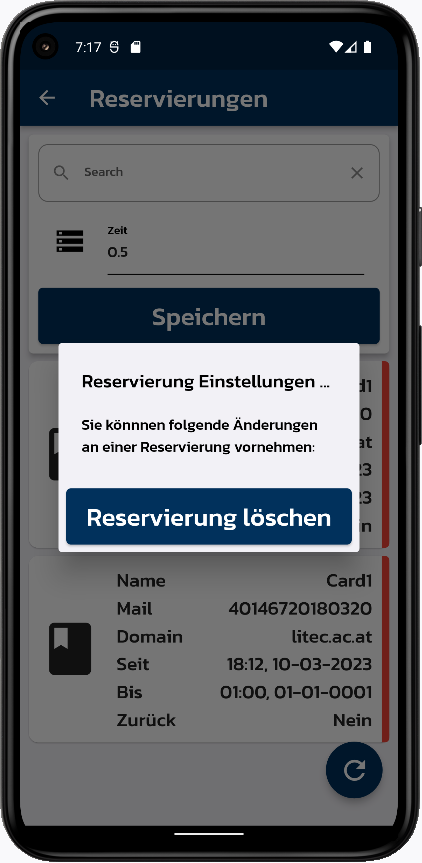
\includegraphics[width=0.4\textwidth]{FLUTTER/images/ZB/reservation_page_selector.png} &
    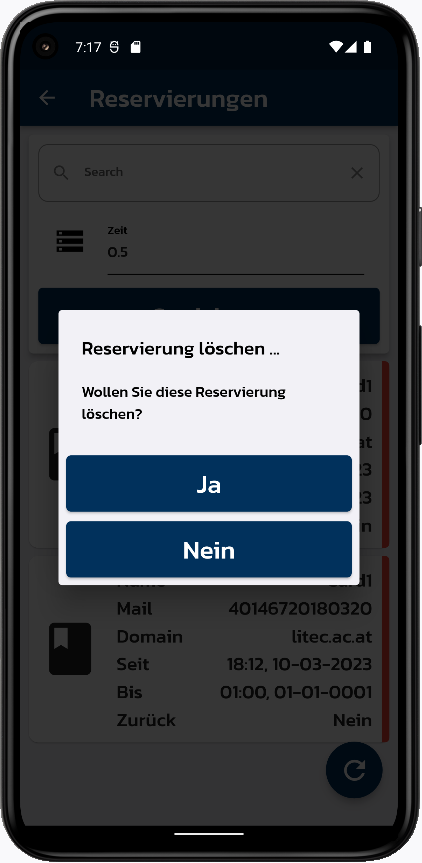
\includegraphics[width=0.4\textwidth]{FLUTTER/images/ZB/reservation_delete.png} \\
  \end{tabular}
  \label{tab:example}
  \captionsetup{type=figure}
  \caption{Reservierung löschen}
\end{table}

\newpage

\subsubsection{Reservierung – Zeit} \label{subsubsec:reservationTime}
Falls die Zeit der spätesten Abholung der Reservierung geändert werden soll, kann dies über die Textbox auf der Reservierung-Seite tun. Die Zeit in Stunden eintrage und ``Speicher`` klicken.

\vspace{1cm}
\begin{table}[htbp]
  \centering
  \begin{tabular}{cc}
    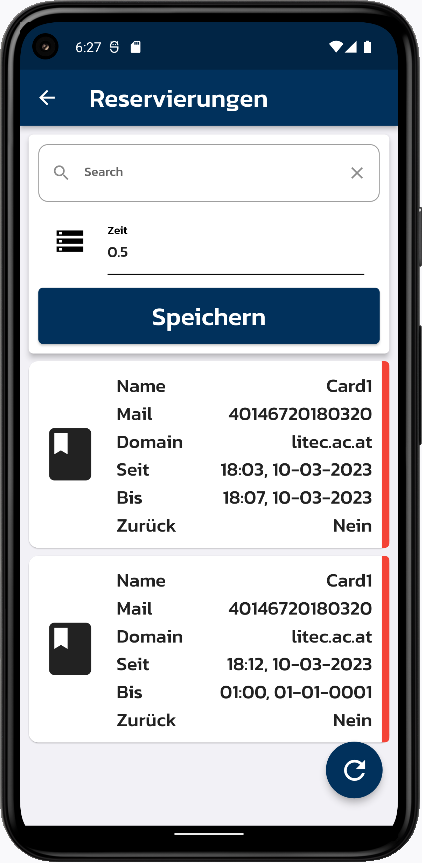
\includegraphics[width=0.4\textwidth]{FLUTTER/images/ZB/reservation_page.png} &
    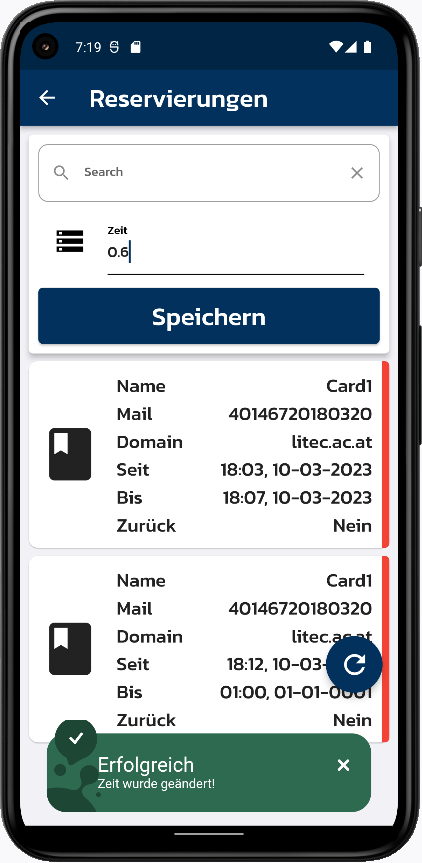
\includegraphics[width=0.4\textwidth]{FLUTTER/images/ZB/reservation_time.png} \\
  \end{tabular}
  \label{tab:example}
  \captionsetup{type=figure}
  \caption{Reservierung Zeit einstellen}
\end{table}

\newpage

\newpage

\subsection{Einstellungen}
Eine der unspektakulären Seiten, welche ebenfalls über die App Bar zugänglich ist, ist die Einstellungs-Seite. Diese erreicht man über Anklicken des Zahnrad Icons. Dort kann der Admin das Theme der App einstellen und der User kann sich abmelden.

\vspace{1cm}
\begin{table}[htbp]
  \centering
  \begin{tabular}{cc}
    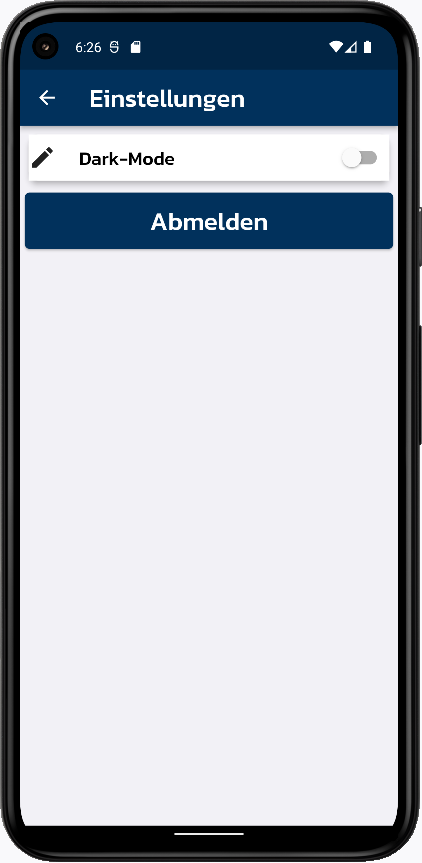
\includegraphics[width=0.45\textwidth]{FLUTTER/images/ZB/settings_page.png} \\
  \end{tabular}
  \label{tab:example}
  \captionsetup{type=figure}
  \caption{Einstellungen}
\end{table}

\newpage

\subsection{Zur Client-Sicht}
Die letzte, aber wichtige, Funktion der Admin Sicht ist die Wechsel-Funktion. Dies ist über das Verlassen Icon zugänglich und bringt den Admin zurück zur Login Sicht.

\vspace{1cm}
\begin{table}[htbp]
  \centering
  \begin{tabular}{cc}
    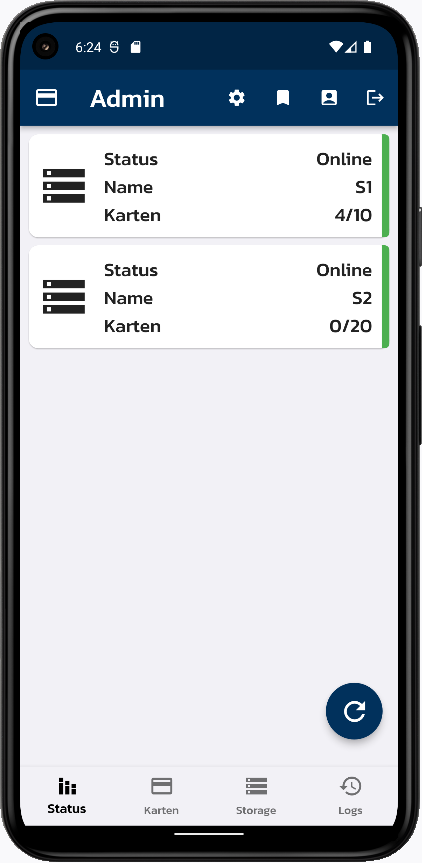
\includegraphics[width=0.4\textwidth]{FLUTTER/images/ZB/status_page.png} \\
  \end{tabular}
  \label{tab:example}
  \captionsetup{type=figure}
  \caption{Zur Client-Sicht}
\end{table}

\newpage

\subsection{Ablauf Diagramm}
Zum Abschluss der Admin Sicht folgt noch ein Ablauf-Diagramm, welches alle Funktion dieser Sicht im Überblick zeigen soll und wie diese zugänglich sind.

\begin{flushleft}
\centering
  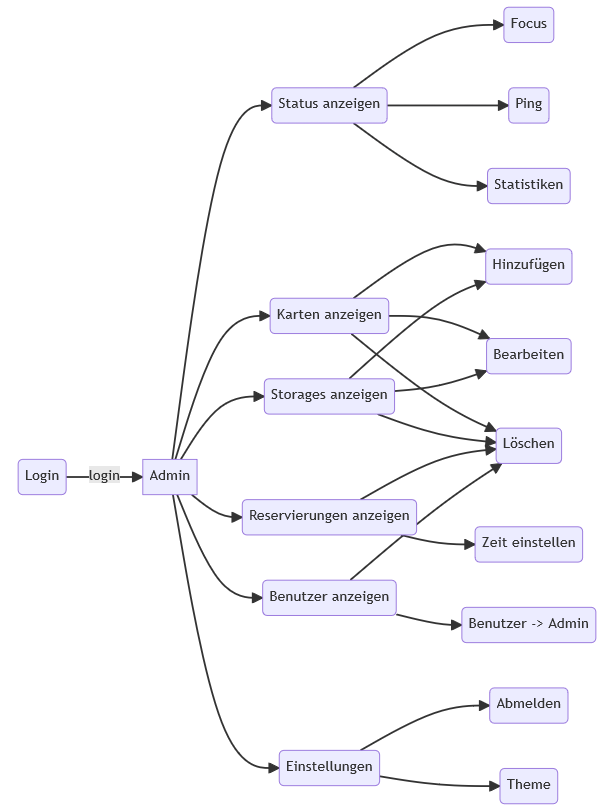
\includegraphics[width=0.85\textwidth]{FLUTTER/images/ZB/admin_flow_diagram.png}
  \captionsetup{type=figure}
  \caption{Ablauf-Diagramm Admin Sicht \cite{Mermaid}}
\end{flushleft}


\newpage
%-----------------------------------------------------
%-----------------------------------------------------
%-----------------------------------------------------
%-----------------------------------------------------
%-----------------------------------------------------
\GpSec{Client Sicht }\label{sec:userguider:clientview}

Der folgende Abschnitt behandelt die Bedienung der Client Sicht. Eine kurze Zusammenfassung ist im Abschnitt {\ref{subsec:thero:client}} aufzufinden.

\subsection{Karten Seite}\label{subsec:kartenseite}

Zum Darstellen der Karten wurde eine eigene Seite erstellt, welche das Ausborgen sowie Reservieren einer Karte ermöglicht. Jede Karte wird in einer eigenen Karteikarte dargestellt, wobei Information wie derzeitiger Verfügbarkeit-Status, Name angezeigt werden. Ebenfalls ist es möglich, jede Karte mittels des {\textit{Stern Button}} zu favorisieren, um einen schnelleren Zugriff zu ermöglichen. 
\begin{figure}[h!]
\centering
    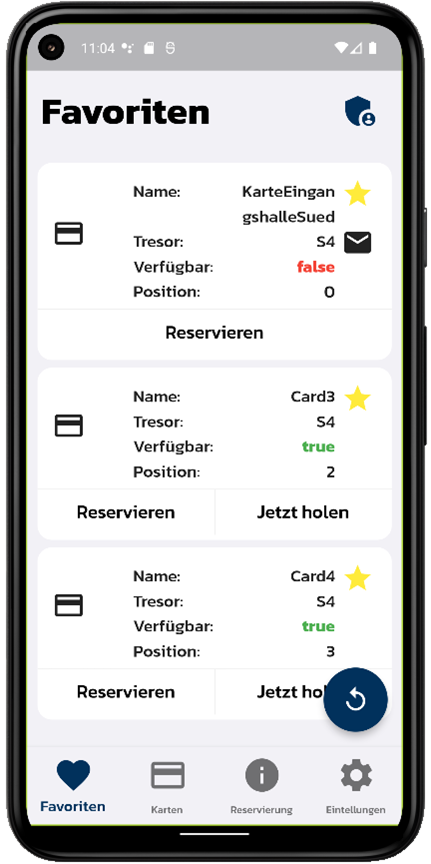
\includegraphics[width=0.39\textwidth]{FLUTTER/images/GP/Client_Karten.png}
    \caption{Navigationsseiten der App}
    \label{fig:navigationsseiten}
\end{figure}
\newpage



\subsubsection{Reservierung einer Karte}


Mittels den {\textit{Reservieren-Button}} können Ihre gewünschten Reservierungen durchgeführt werden, wobei dessen Gültigkeit (Keine Reservierung(en) in den gewünschten Zeitraum vorhanden), überprüft wird. Ist eine Reservierung durchgeführt worden, aktiviert sich ein Benachrichtigungsservice, welche den Benutzer über eine bevorstehende Reservierung aufmerksam macht.


\begin{table}[htbp]
  \centering
  \begin{tabular}{cc}
    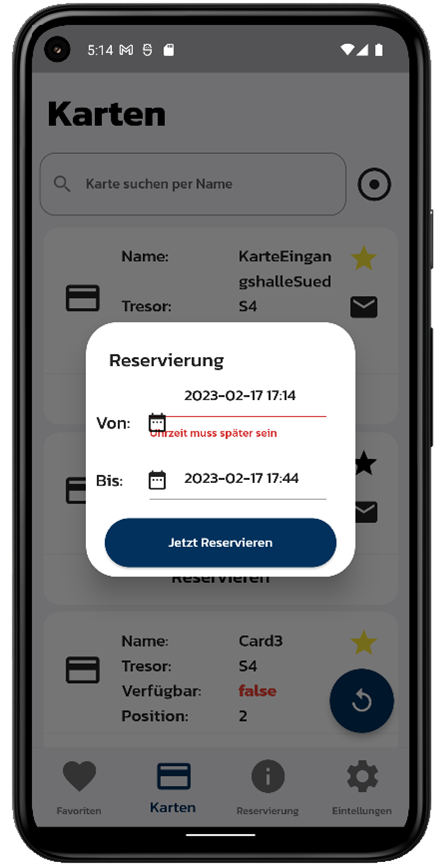
\includegraphics[width=0.4\textwidth]{FLUTTER/images/GP/Client_Reservation.png} &
    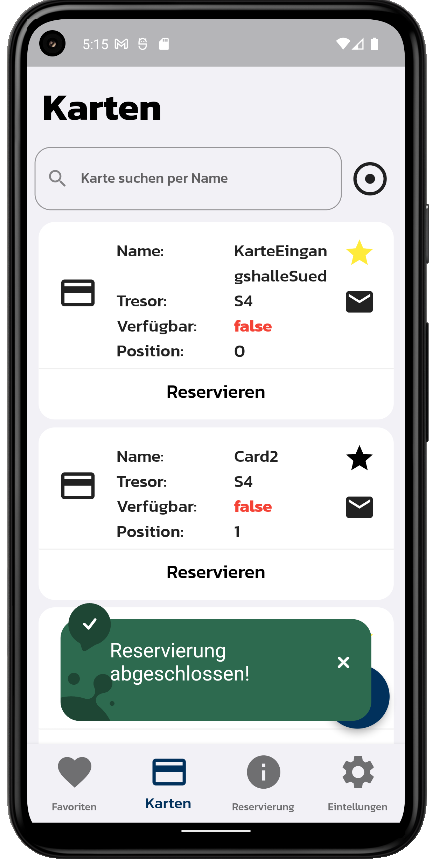
\includegraphics[width=0.4\textwidth]{FLUTTER/images/GP/Client_Reservation_Success.png} \\
  \end{tabular}
  \caption{Ablauf einer Reservierung}
  \label{tab:example}
\end{table}

\newpage
\subsubsection{Anforderung einer Karte}
Ebenfalls werden die Buttons der Karte dynamisch generiert. Somit wird nur dann die Möglichkeit geboten, eine Karte auszuborgen, wenn diese gerade nicht in Benutzung ist. Um eine Karte anzufordern, drücken Sie den Button {\textit{Jetzt holen}} und Ihre Karte wird beim entsprechendem Tresor heruntergelassen. Ebenfalls wird Ihnen bei einer erfolgreichen Anforderung eine Reservierung hinzugefügt und ein Feedback-Dialog erscheint.
\begin{figure}[!h]
\centering
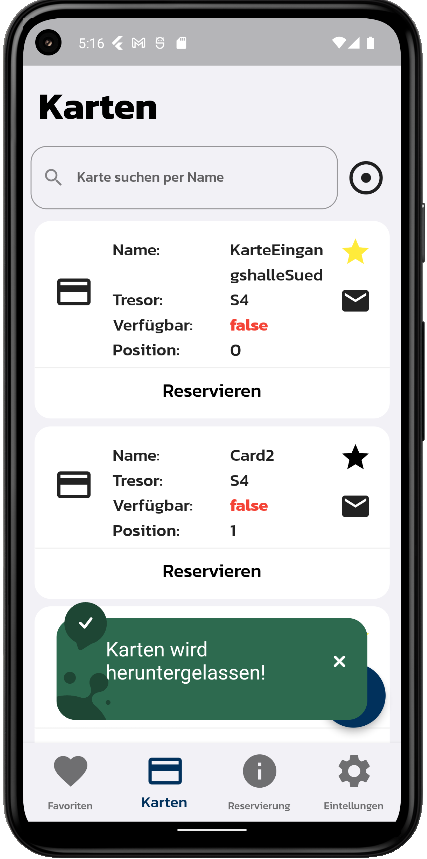
\includegraphics[width=0.4\textwidth]{FLUTTER/images/GP/Client_Get_Card.png}
\caption{Karte anforden}
\end{figure}
\newpage


\subsubsection{Senden einer Mail bei Verwendung}
Falls die Karte nun in Verwendung ist, gibt es die Funktion mittels den {\textit{Post Button}}, die aktuelle Person, die die Karte verwendet eine Mail zu schreiben. Hierbei öffnet sich ein Pop-Up, welches die installierten Mail-Apps bspw. Outlook anzeigt. Hat sich der Nutzer, für eine Mail App entschieden, öffnet sich ein bereits ausgefülltes Fenster (E-Mail Benutzer, Begrüßung und, usw.) um eine E-Mail zu versenden.

\begin{figure}[!h]
\centering
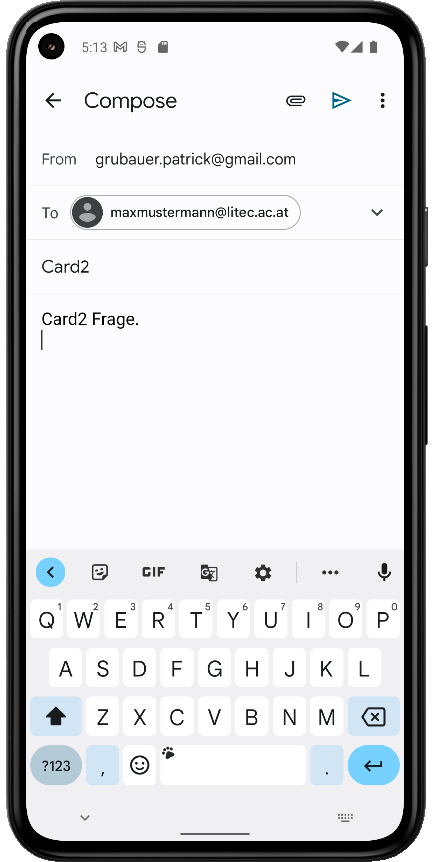
\includegraphics[width=0.4\textwidth]{FLUTTER/images/GP/Cleint_Send_Mail.png}
\caption{Vorausgefüllter Mailentwurf}
\end{figure}

\newpage
\subsection{Favoriten Seite}
Trotz einer Filter –und Suchfunktion, kann bei besonders vielen Karten schnell der Überblick verloren gehen. Lösung dafür war eine Favoriten-Seite. Diese ermöglicht eine schnellere und effektivere Möglichkeit, Karten aufzufinden.\\ 
Die Favoriten-Seite ist eine Erweiterung der \nameref{subsec:kartenseite}. Sie beinhaltet dieselben Eigenschaften, wie die \nameref{subsec:kartenseite} unter Bedienung, dass die Karten favorisiert worden sind (sternförmiges Zeichen gelb). Durch eine Wiederbetätigung des Buttons erfolgt eine Entfavorisierung.
\begin{figure}[!h]
\centering
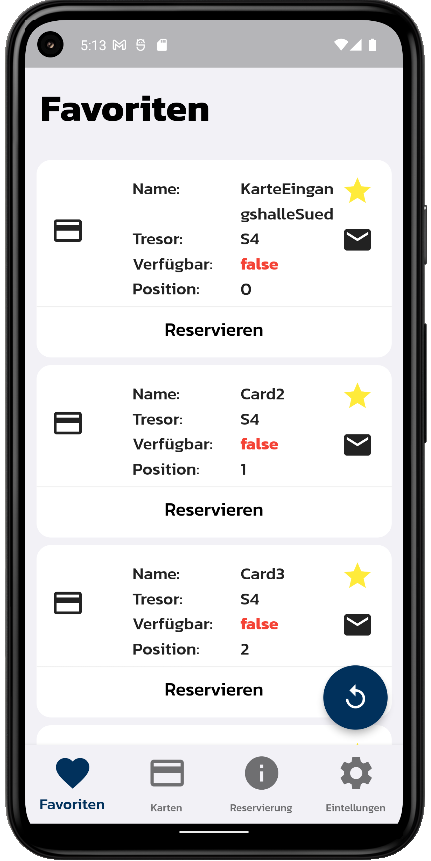
\includegraphics[width=0.4\textwidth]{FLUTTER/images/GP/Client_Favorite.png}
\caption{Favoriten Seite}
\end{figure}



\newpage
\subsection{Reservierungen}
Diese Seite stellt alle Karten, die vom Benutzer reserviert oder ausgeborgt worden sind, dar. Es werden wie bei der \nameref{subsec:kartenseite} ebenfalls alle Informationen einer Reservierung mittels einer Karteikarte angezeigt. Wobei zusätzlich, der Start -sowie Endzeitpunkt einer Reservierung mitgeteilt wird. Falls der Endzeitpunkt unbekannt ist, wird die Karte derzeit verwendet und das Feld für den Endzeitpunkt bekommt den Wert {\textit{In Benutzung}}.\\
Der genaue Ablauf der Generierung der Karten wird im Kapitel \ref{subsec:impl:visualizeapidata} beschrieben.

\begin{table}[htbp]
  \centering
  \begin{tabular}{cc}
    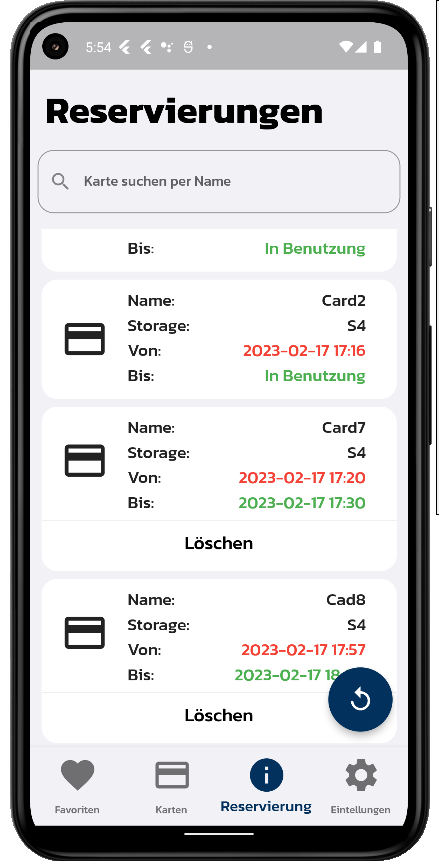
\includegraphics[width=0.4\textwidth]{FLUTTER/images/GP/Client_Reservation_Site.png}&
    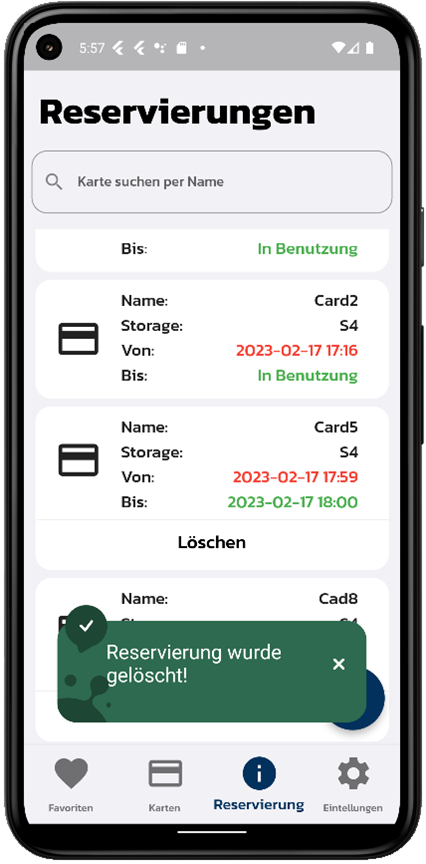
\includegraphics[width=0.4\textwidth]{FLUTTER/images/GP/Client_Reservation_Site_Delete.png} \\
  \end{tabular}
  \caption{Reservierungen anzeigen und l\"oschen}
  \label{tab:example}
\end{table}

%\begin{figure}[h!]
%\centering
%%\subfigure[Reservierungen Seite]{\includegraphics[width=0.4\linewidth]%{FLUTTER/images/GP/Client_Reservation_Site.png}}
%%\subfigure[Reservierung löschen]{\includegraphics[width=0.4\linewidth]%{FLUTTER/images/GP/Client_Reservation_Site_Delete.png}}
%\caption{Reservierungen bearbeiten und anzeigen}
%\end{figure}

\newpage
\subsection{Einstellungen}

Diese Seite wurde erstellt, um dem Benutzer die Möglichkeit zu geben, die Funktionsweise und das Auftreten der App je nach Bedürfnisse anzupassen.
\begin{figure}[!h]
\centering
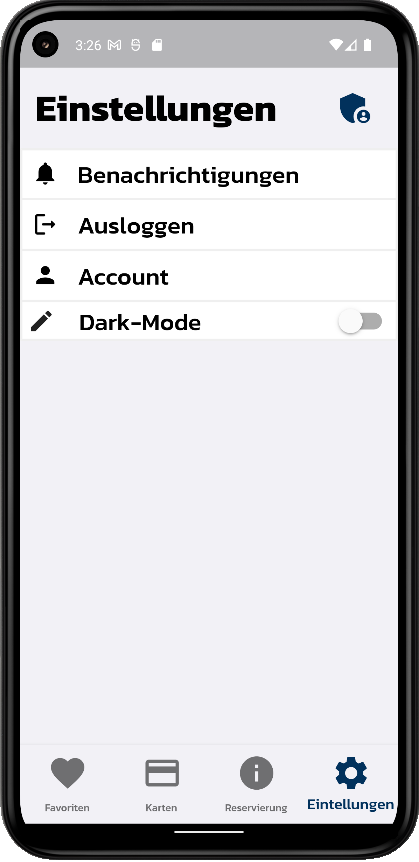
\includegraphics[width=0.4\textwidth]{FLUTTER/images/GP/Client_Einstellungen.png}
\caption{Einstellungen}
\end{figure}
\newpage
\subsubsection{Benachrichtigung}
Dieser Button ermöglicht dem Benutzer, Benachrichtigungen der Applikation deaktivieren zu können. Hierbei öffnen sich die {\textit{Einstellungen}} des verwendeten Betriebssystems mit einer direkten Weiterleitung auf die Einstellung der Benachrichtigungen unserer App.
\begin{figure}[!h]
\centering
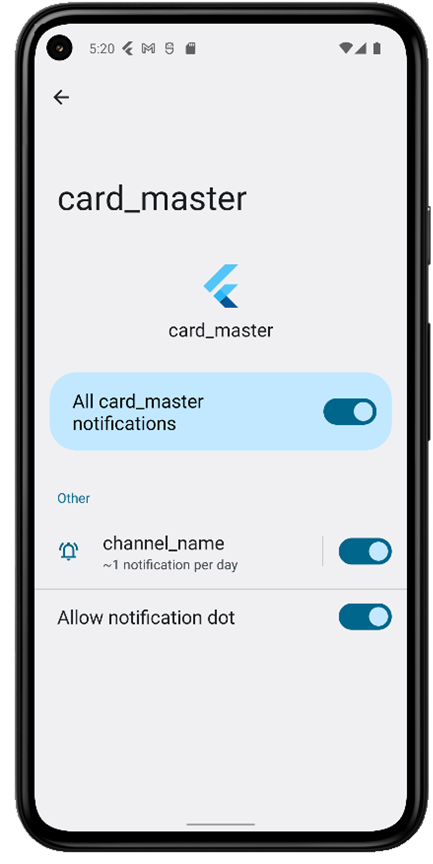
\includegraphics[width=0.4\textwidth]{FLUTTER/images/GP/Notification.png}
\caption{Benachrichtigung einstellen}
\end{figure}
\newpage

\subsubsection{Account}
Um sich einen Überblick über den derzeit eingeloggten Benutzer zu verschaffen wurde eine Account-Seite erstellt, welche verschiedene Informationen wie E-Mail, Name, usw. repräsentiert.
\begin{figure}[!h]
\centering
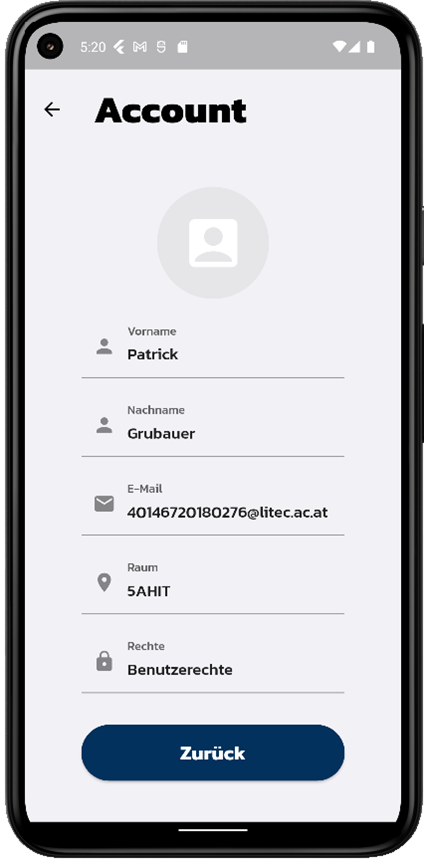
\includegraphics[width=0.4\textwidth]{FLUTTER/images/GP/Account.png}
\caption{Account Seite}
\end{figure}

\newpage

\subsubsection{Dark Mode Funktion}
Hierbei handelt es sich um einen Switch Button, der wenn aktiv den {\textit{dunklen Modus}} der App aktiviert. Weiters wird dieser Status gespeichert, damit beim Neustart das bevorzugte Theme verwendet wird. Die genaue Funktionsweise wird im Abschnitt \ref{subsec:impl:themehandler} beschrieben
\begin{figure}[!h]
\centering
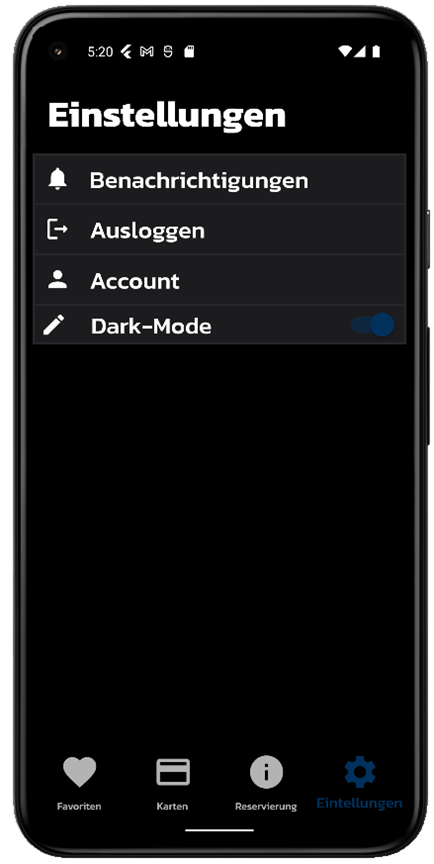
\includegraphics[width=0.4\textwidth]{FLUTTER/images/GP/Dark_Mode.png}
\caption{Dunkler Modus Funktion}
\end{figure}

\newpage

\subsubsection{Ausloggen}
Mittels dieses Buttons wird der Benutzer abgemeldet und gelangt an die \ref{sec:userguider:loginview} \nameref{sec:userguider:loginview}. Ebenfalls erfolgt die Löschung aller gespeicherten Daten.

\subsection{Sonstiges}
\subsubsection{Such –und Filtermöglichkeiten}
Um eine bestimmte Karte schneller zu finden, gibt es neben der {\textit{Favoriten-Seite}} ebenfalls die Möglichkeit eine Karte oder Reservierung mit der Such – und Filterfunktion aufzufinden. Die Filterfunktion kann nach den gewünschten Tresornamen und dem Verfügbarkeit-Status filtern, wobei die Suchfunktion die Karten anhand der Kartenbenennung durchsiebt
\begin{table}[htbp]
  \centering
  \begin{tabular}{ccc}
    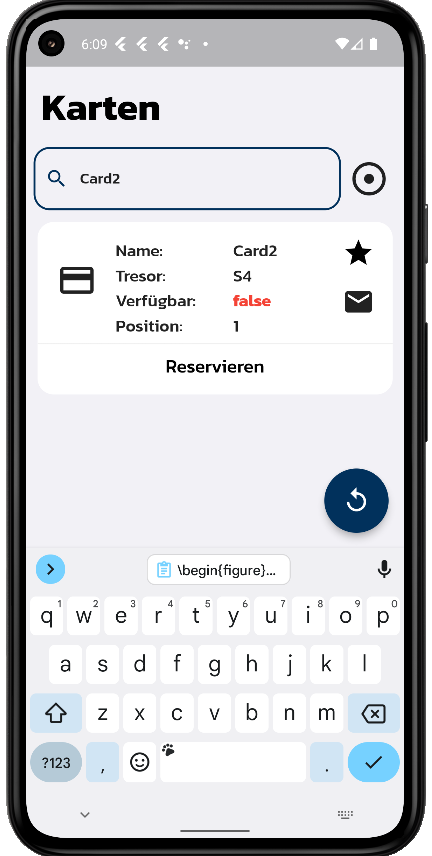
\includegraphics[width=0.3\textwidth]{FLUTTER/images/GP/Search.png}&
    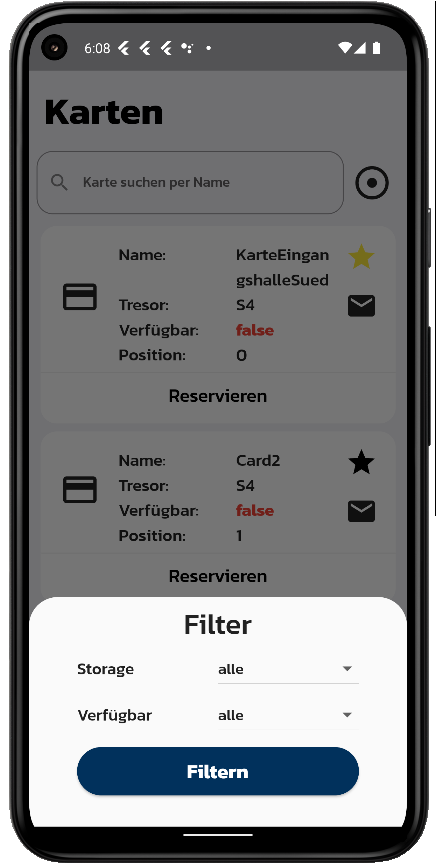
\includegraphics[width=0.3\textwidth]{FLUTTER/images/GP/Filter.png}
    \\
  \end{tabular}
  \captionsetup{type=figure}
  \caption{Such –und Filtermöglichkeiten}
  \label{tab:example}
\end{table}

\newpage

\subsubsection{Adminrechte}
Je nach Zugriffsrechten ist es möglich, dass ein Benutzer über Adminrechte verfügt. Unter dieser Bedingung erscheint bei der Kopfzeile der App ein Button, welcher bei Betätigung zur Administratoransicht wechselt, siehe {\textit{\nameref{fig:navigationsseiten}s}}

\subsection{Ablaufdiagramm}
Die Funktionalität der App anhand einer simplen Grafik.
\begin{figure}[h]
\centering
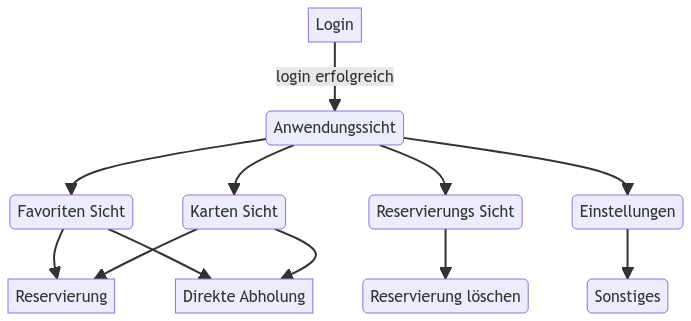
\includegraphics[width=1.0\textwidth]{FLUTTER/images/GP/mermaid-client.png}
\caption{Ablaufdiagramm Client–Sicht}
\end{figure}

\newpage
\GpSec{Login–Sicht }\label{sec:userguider:loginview}
Der folgende Abschnitt behandelt die Bedienung der Login Sicht. Eine kurze Zusammenfassung ist im Abschnitt \ref{subsec:thero:login} \nameref{subsec:thero:login} aufzufinden.

\subsection{Eingeloggt bleiben Funktion}
Diese Funktion ermöglicht dem Benutzer bei der Anwendung angemeldet zu bleiben. Dies spart Zeit und verbessert somit die Benutzerfreundlichkeit, da die Abfrage der Informationen des Nutzers bei Neustart der Anwendung nicht durchgef\"uhrt werden muss.
\begin{figure}[!h]
\centering
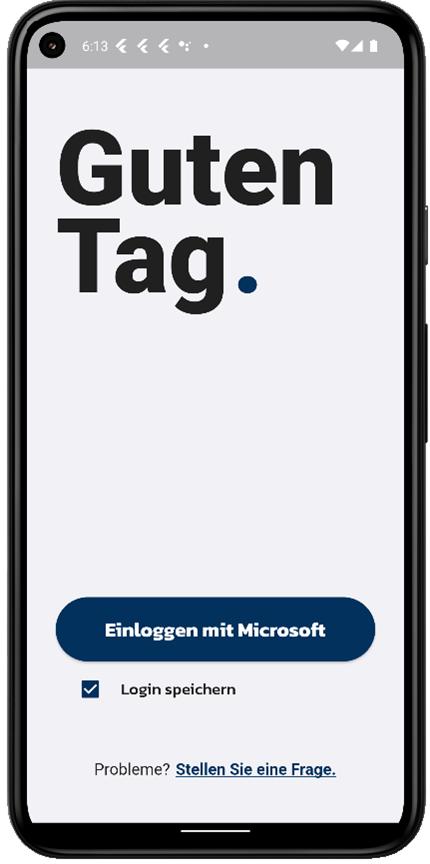
\includegraphics[width=0.4\textwidth]{FLUTTER/images/GP/Login_Allg.png}
\caption{Login Sicht}
\end{figure}

\newpage
\subsection{Report Möglichkeit}
Falls der Benutzer Fragen oder Probleme bei der Benutzung der Applikation hat, kann er dem Support eine Mail schreiben. Beim Dr\"ucken des blau hervorgehobenen Text öffnet sich, je nach Auswahl der Mail App, ein vorausgefülltes Fenster zum Schildern des Problems. 
\begin{figure}[h]
\centering
\includegraphics[width=0.4\textwidth]{FLUTTER/images/GP/Login_QAA.png}
\caption{Frage an Support}
\end{figure}


\newpage
\subsection{Login via Microsoft}
Die {\textit{Login mit Microsoft} Funktion ermöglicht dem Benutzer die Registrierung bei der Anwendung über ein Microsoft Konto. Aufgrund des Domain-Namens {\textit{litec.ac.at}} kann sichergestellt werden, dass es sich wirklich um eine Person des Linzer Technikums handelt. Ebenfalls ist es nun nicht mehr unsere Aufgabe, die Anmeldedaten des Benutzers sicher zu speichern, da Microsoft verpflichtet ist, die Datenschutzrechte seiner Benutzer einzuhalten.

\begin{figure}[!h]
\centering
\includegraphics[width=0.4\textwidth]{FLUTTER/images/GP/Login_Micro.png}
\caption{Login mit Microsoft}
\end{figure}

\newpage

\subsection{Registrierungsvorgang}\label{subsec:Registrierungsvorgang}
Um einen Benutzer vollständig registrieren zu können, werden zwei Informationen benötigt. Die E-Mail des Nutzers, sowie die Informationen, welche auf der Druckerkarte des Professors gespeichert sind. Beide Informationen werden beim Registrierungsvorgang abgefragt. Wie der Registrierungsvorgang implementiert wurde, wird im Abschnitt  \ref{subsec:impl:login} \nameref{subsec:impl:login} erklärt.
\\Es erfolgt eine kurze Erklärung des Registrierungsvorgangs.

{\textbf{Hinweis:}} Die Registrierung am Smartphone ist die einzige Methode, einen Benutzer in das System aufzunehmen. Die Registrierung direkt am Tresor, wäre unmöglich, da der Internetzugang zum Tresor aufgrund von Sicherheitslücken untersagt wurde. 
\begin{itemize}
    \item Einloggen mit Microsoft.
    \item Auswahl des zu verwendenden Tresors, bzw. dessen Kartenlesegeräts.
    \item Erscheinen eines Timer-Dialogs, welcher die verfügbare Zeit darstellt.
    \item Karte an Lesegerät halten.
    \item Registrierung abgeschlossen.
\end{itemize}

   
\begin{table}[htbp]
  \centering
  \begin{tabular}{ccc}
    \includegraphics[width=0.2\textwidth]{FLUTTER/images/GP/Login_Select_Storage.png}&
    \includegraphics[width=0.2\textwidth]{FLUTTER/images/GP/Login_timer.png}&
    \includegraphics[width=0.2\textwidth]{FLUTTER/images/GP/Login_register_sucees.png}
    \\
  \end{tabular}
  \captionsetup{type=figure}
  \caption{Ablauf der Registrierung}
  \label{tab:example}
\end{table}

\newpage

\subsubsection{Ablaufdiagramm der Registrierung}
Der Ablauf einer Registrierung anhand einer simplen Grafik.
\begin{figure}[h!]
\centering
\includegraphics[width=0.7\textwidth]{FLUTTER/images/GP/LoginAblaufAllgEPK.png}
\caption{EPK Diagramm Login–Sicht}
\end{figure}


\newpage
\subsection{Funktionsdiagramm}
Die Funktionalit\"at der Login Sicht anhand einer simplen Grafik.
\begin{figure}[h!]
\centering
\includegraphics[width=0.9\textwidth]{FLUTTER/images/GP/login_funktion.png}
\caption{Funktionsdiagramm Login–Sicht}
\end{figure}
\newpage

\GpSec{Display Anwendung Raspberry }\label{sec:userguider:displayview}
Der folgende Abschnitt behandelt die Bedienung der Display-Sicht am Tresor. Eine kurze Zusammenfassung ist im Abschnitt \ref{subsec:thero:display} \nameref{subsec:thero:display} aufzufinden.

\subsection{Anforderung einer Karte}
Wie bereits in der Einleitung erklärt wurde, ist es möglich als {\textbf{registrierter}} Benutzer eine Karte am Terminal anzufordern.
\begin{figure}[!h]
\centering
\includegraphics[width=1\textwidth]{FLUTTER/images/GP/Display_Allg.png}
\caption{Display Karten Seite}
\end{figure}

\newpage
Allerdings wird die Kartennummer, welche bei der Registrierung \ref{sec:userguider:loginview} des Benutzers gespeichert wurde, zur Identifizierung des Nutzers verwendet, indem er diese beim Anfordern der Karte, mit dem Kartenlesegeräts des Tresors scannen lässt. Dazu erscheint ein Pop-Up am Display, welches dem Benutzer die restliche Zeit zum Authentifizieren bzw. Scannen der Karte anzeigt. 


\begin{figure}[!h]
\centering
\includegraphics[width=1\textwidth]{FLUTTER/images/GP/Display_Timer.png}
\caption{Display Anwendung Timer}
  \label{fig:display:timer}
\end{figure}

\newpage
Ist der Benutzer bereits registriert, wird die Karte heruntergelassen und dem Benutzer wird eine Reservierung hinzugefügt. Falls die Zeit nun abgelaufen ist oder eine Karte eines nicht registrierten Benutzers gescannt wurde, erscheint ein Pop-Up \ref{feedbackdialog} mit einer Fehlernachricht. Diese könnte wie folgt aussehen:  
\begin{figure}[!h]
\centering
\includegraphics[width=1.0\textwidth]{FLUTTER/images/GP/Display_Warning.png}
\caption{Pop-Up bei abgelaufener Authentifizierungszeit am Tresordisplay}
  \label{fig:display:popup}

\end{figure}

{\textbf{Hinweis:}} Dieses Pop-Up wurde implementiert, um den Ablauf aller Prozesse des Clients -, Login – und Display Anwendung zu überwachen. Es wird bei jeder Aktion angezeigt, um zu gewährleisten, dass alle Informationen über den Verlauf der Prozesse aufgezeichnet werden. Die genauere Beschreibung der Implementierung und der verschiedenen Arten von Pop-ups, erfolgt im Abschnitt \ref{feedbackdialog} \nameref{feedbackdialog}

\newpage
\subsection{Anzeigen der Reservierungen}
Ebenfalls ist es mo\"glich, die derzeitigen Reservierungen, der Karten, welche im entsprechenden Tresor aufbewahrt wird, anzuzeigen. Hierbei werden Information wie Name, Zeit, usw. angezeigt. Dies ist praktisch, um ein Gefühl dafür zu bekommen, wie viele Reservierungen und Karten derzeit vorhanden sind.
\begin{figure}[!h]
\includegraphics[width=1.0\textwidth]{FLUTTER/images/GP/Display_Reservation.png}
\caption{Reservierungen Sicht der Display-Anwendung}
\end{figure} %ja
\subsection{Anzeigen eines Dialogs bei einer Registrierung}
Eine weitere wichtige Eigenschaft der Display-App ist das Anzeigen eines Timers bei einer Neuregistrierung. Aufbauend darauf wird je nach Erfolg bzw. Misserfolg ein Dialog angezeigt.
Der Ablauf der Registrierung wird im Abschnitt \ref{sec:userguider:loginview} erklärt. 
\begin{itemize}
    \item Der Nutzer wählt bei der Neuregistrierung einen Tresor aus, um seine Karte scannen zu lassen. Während des Scann-Vorgangs erscheint ein Pop-Up am Display, welches die restliche Zeit zum Scannen der Karte anzeigt, siehe Abbildung \ref{fig:display:timer}.
    \item Bei einer erfolgreichen oder nicht erfolgreichen Registrierung wird ein Pop-Up angezeigt, siehe Abbildung \ref{fig:display:popup}
\end{itemize}
\subsection{Sonstiges}
Um eine bestimmte Karte oder Reservierung schneller zu finden, gibt es die Möglichkeit diese mit einer Filterfunktion aufzufinden. Die Filterfunktion wird oben rechts angezeigt und kann nach dem gewünschtem Verfügbarkeitsstatus der Karte sowie Name, welche im entsprechenden Tresor gelagert sind, filtern.
\begin{figure}[!h]
\includegraphics[width=1.0\textwidth]{FLUTTER/images/GP/Display_Filter.png}
\caption{Filter-Funktion der Display-Anwendung}
\end{figure}
\newpage
\subsection{Funktionsdiagramm}
Die Funktionalität der Anwendung anhand einer simplen Grafik.
\begin{figure}[!h]
\centering
\includegraphics[width=1\textwidth]{FLUTTER/images/GP/display_anwendung_ablauf.png}
\caption{Ablaufdiagramm Display Anwendung}
\end{figure}